\documentclass{article}
\usepackage{amsmath}
\usepackage{graphicx}
\usepackage[capitalize]{cleveref}
\begin{document}
\section{General discussion}
We want to study a simple model of demography. The central object of interest is the number of people at age $n$, which we measure in days. Let us for simplicity first neglect sex, such that the state is encoded in the vector $A$ whose components $A_n$ give the number of people which are $n$ days old. This vector is finite dimensional, as one can expect that age is bounded from above by at least $150*365 = 54750$. 

Additionally, the state vector is a function of time $A(t)$, where time is discretized in days as well, such that we can model the dynamics. In order to do so we account for the following processes:
\begin{itemize}
\item Aging: everyday, everyone ages by one day
\item Birth: everyday, some number of people is born, i.e. added into the $A_0$ group
\item Death: everyday, some number of people at all ages die, i.e. are taken away from the corresponding age group
\end{itemize}
We formalize this in terms of the following equation:
\begin{equation}
	A_n\left(t+1\right) = 
	\begin{cases}
		\left\{1 - D_n\left[t,A\right]\right\}A_{n-1}\left(t\right) \quad \text{for} \quad n>0 \\
		B\left[t,A\right] \quad \text{for} \quad n=0
	\end{cases}
\end{equation}
where $B$ denotes the number of births and $D_n$ denotes the probabilty to die at age $n-1$. Note that the whole problem lies in the question of how to model the dependence of death and birth rates on time and the total demography (possibly also at earlier times!). We will discuss various realizations in the following, gradually increasing the level of complexity.

\subsection{Simplest model: certain death beyond a given age, constant birth rates}
The simplest model one can think of is given by setting a certain constant birth rate $B_0$ and an age $n_D$, after which death is certain:
\begin{equation}
	D_n = 
	\begin{cases}
		0 \quad \text{for} \quad n<n_D \\
		1 \quad \text{for} \quad n\geq n_D \\
	\end{cases}
\end{equation}
\cref{fig:model1} shows the dynamic of this simple model.
\begin{figure}
	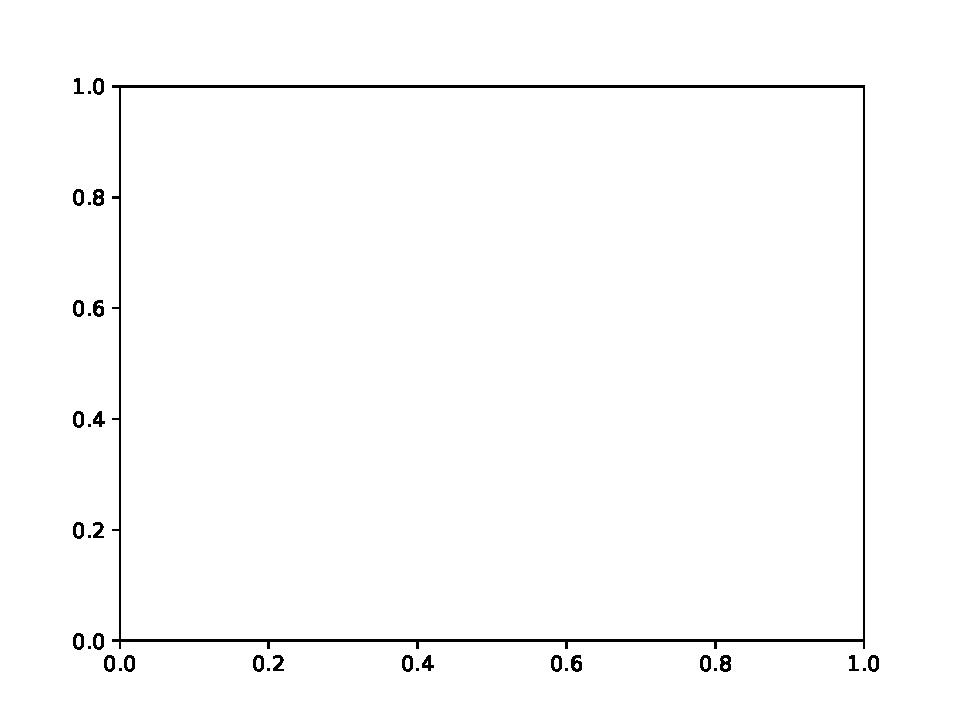
\includegraphics[width=\textwidth]{figures/model1.pdf}
	\caption{Dynamics of the simplest model with constant birth rates and certain death age, starting from a random distribution. \label{fig:model1}}
\end{figure}

\end{document}
